\documentclass[10pt]{article}
% Puedes usar esto (u otra codificaci\'on) si quieres:
\usepackage{graphicx}
\usepackage[utf8]{inputenc} %para usar acentos por ejemplo
\usepackage[spanish]{babel}  % para que las directivas del latex se impriman en españos. Por ejemplo \begin{abstract} ... \end{abstract}, aparecería "Abstract", pero con este paquete aparecerá "Resumen"
\usepackage{imakeidx}
\usepackage{listings}
\usepackage{float}
\usepackage{hyperref}

\makeindex[columns=3]

\title{Optimizacion en la Industria} % El titulo debería ser lo mas descriptivo y conciso posible
\author{Rosas Francisco, Gurruchaga Luciano}

\date{\today} % Eliminar \today y no pone la fecha actual según se indica: \date{}

\begin{document}

% Agrega el título
\maketitle

\begin{abstract}
En el presente informe se realizara una breve introduccion al problema de Strip Packing \textbf{SPP} y a los algoritmos geneticos \textbf{GA}, primero daremos una descripcion superficial tanto de SPP como de GA, seguido de una descripcion formal de SPP junto a un problema particular, luego, definiremos formalmente los GA y lo aplicaremos al problema anterior, se realizaran dos implementaciones distintas y una comparativa de los mismos a la hora de resolver el problema. 

\end{abstract}

%----------------------------------------------------------------------------------------
%	Contenido del artículo
%----------------------------------------------------------------------------------------

\section{Introducción}


Los Algoritmos Geneticos conocidos como GA por sus siglas en ingles Genetic Algorithm, son una analogía a la selección natural, es decir, que estan inspirados en ella.

\t Se trabaja con un conjunto de soluciones al que llamaremos \textbf{poblacion}, cada solucion particular o \textbf{individuo} es representada por medio de un vector de valores discretos llamado \textbf{cromosomas}. A los simbolos que conforman dichos vectores se les llama \textbf{genes}. Los cromosomas evolucionan a lo largo de distintas iteraciones, las llamadas \textbf{generaciones}. En cada generacion, los cromosomas son evaluados usando alguna medida de aptitud o funcion objetivo. Las siguientes generaciones, nuevos cromosomas, son generadas aplicando operadores genéticos repetidamente a la generacion actual, siendo estos los operadores de selección (selection), cruzamiento (crossover), mutación (mutation) y reemplazo.

\t El problema de empaquetamiento de tiras SPP del ingles Strip Packing Problem, es un problema de minimización geométrica bidimensional.

\t Dado un conjunto de rectángulos alineados con el eje y una tira de ancho acotado y altura infinita, se busca determinar un empaque sin superposición de rectángulos en la tira de forma tal que se minimice la altura.

\section{Descripción del Problema}
En el problema  de Strip Packing (SPP) o empaquetado de tiras bidimensionales tenemos, una tira de anchura finita W pero de altura infinita, y un conjunto de elementos rectangulares de anchura máxima W. 
	El objetivo es empaquetar todos los elementos en la tira para minimizar la altura utilizada. Los elementos no pueden solaparse ni girarse(estudiaremos un caso en el que si puedan rotar). 
Dentro del mismo nivel, todos los elementos se empaquetan de forma que sus fondos queden alineados. El primer nivel es el fondo de la tira y los niveles siguientes se definen por la altura del artículo más alto del nivel anterior.
	Este es un problema de mucho interes de estudio ya que forma parte del a familia de problemas $NP-Hard$, es decir no se ha encontrado una solución en un tiempo polinomico.

\subsection{Definicion:}
%$  X  $
Una instancia $ I = (R,W)$  del problema de empaquetado de tiras consiste en una tira con anchura $W = 1$ y altura infinita, así como un conjunto $R$  de elementos rectangulares. Cada elemento $r   \in   R$ tiene una anchura  $w_r \in  (0,1]  \cap  Q $ y una altura  $h_r     \in   (0,1] \cap Q $. Un empaquetamiento de los elementos es un mapeo en cada esquina inferior izquierda de un elemento $r    \in   R$  a una posición $(x_r,y_r) \in([0,1 - w_r] \cap Q) \times Q\geq 0$ en el interior de la franja. 
Un punto interior de un elemento colocado $ r \in  R $ es un punto del conjunto $inn(r)={(x,y) \in Q\times Q | x_r < x_r + w_r , y_r<y_r+h_r}$ .
Dos elementos (colocados) se solapan si comparten un punto interior. La altura del empaquetamiento se define como $ \max \{ y_r + h_r | r \in R\} $. El objetivo es encontrar un empaquetamiento libre de solapamiento de los elementos dentro de la franja minimizando la altura del empaquetamiento.

 En este informe utilizaremos una serie de instancias 
contenidas en ("spp9a.txt", "spp9b.txt", "spp10.txt", "spp11.txt", "spp12.txt", "spp13.txt") las cuales varian en su conjunto $R$ y en $W$.

\section{Propuesta algorítmica} % El titulo de esta y el resto de las secciones es orientativa

\t Una forma comun de atacar este problema es el enfoque orientado al nivel, los rectangulos se insertan de izquierda a derecha, en filas que forman niveles. Dentro del mismo nivel, todos los elementos se empaquetan de forma que sus fondos se alineen. El primer nivel es el fondo de la tira y los niveles siguientes se definen por la altura del rectangulo más alto del nivel anterior.
 
\t Algunos algoritmos comienzan ordenando los artículos por altura no creciente, suelen denominarse de altura decreciente \textbf{DH}, y orientados al nivel. Varaciones de dicho algoritmo son los algoritmos First-Fit Decreasing Height \textbf{FFD}, Next-Fit Decreasing Height \textbf{NFD} y Best-Fit Decreasing Height \textbf{BFDH}.[5]

Existen muchas mas variaciones, nosotros utilizaremos un enfoque orientado al nivel, pero en vez de ordenar los elementos por su altura, utilizaremos un enfoque metaheuristico poblacionall, mas precisamente un algoritmo genetico que encuentre una solucion aproximada aceptable a nuestro problema.

\subsection{¿Que es un Algoritmo Genetico?}

Un algoritmo genetico es una metaheuristica poblacional inspirada en el proceso de la seleccion natural.

Contamos con una poblacion $P$, dicha poblacion esta formada por un conjunto de soluciones individuos $I$, cada individuo $I$ esta representado por un conjunto de cromosomas, los cuales a su vez estan formados una secuencia de genes $g_i$ de valor discreto, que representan una solucion al problema, formalmente:

$$P =\{i_0,i_1,..,i_n\}$$
$$I =\{(g_0,g_1,..,g_n)_0,(g_0,g_1,..,g_n)_1,...,(g_0,g_1,..,g_n)_n\}$$

Se toman todos los individuos de la poblacion $I \in P$, se obtiene una medida de "desempeño" de cada solucion $I$, aquellos con mejor desempeño son mas propensos a reproducirse, como sucede en la seleccion natural donde los mas aptos sobreviven y tienen mas posibilidades de trasmitir sus genes.

Existen distintas formas de seleccionar que individuos se reproducen, nosotros utilizaremos la \textit{"seleccion basada en torneos"} la cual consiste en seleccionar de forma aleatoria dos individuos distintos de la poblacion, y , aquel con mejor desempeño sera quien pueda reproducirse y por tanto sus genes seran "heredados" en la siguiente poblacion $P$. Sumado a esto existe una probabilidad de cruza y mutacion de los genes al reproducirse.

Para la primera utilizaremos el operador de cruce \textbf{PMX} o \textit{cruce por emparejamiento parcial}. Consiste en elegir un subsegmento de los genes de uno de los progenitores y cruzarlos preservando el orden y la posición de la mayor cantidad de genes posible del otro manteniendo la coherencia.
En cuanto a la mutacion utilizaremos una \textit{permutacion simple} entre dos genes aleatorios $g_i,g_j$ del mismo individuo.

A medida que avanzan las generaciones, en cada poblacion iran quedando aquellos individuos que cuentan con los "mejores"  genes de generaciones anteriores, por tanto los de mejor desempeño. Recuperando al mejor individuo historico (de todas las generaciones) obtenemos una solucion aproximada aceptable.

\subsection{Aplicacion a SPP}
En nuestro caso particular contaremos con diferentes $(R,W)$ por achivo. Los cuales representan un $W$ y serie de rectangulos $r_i \in R$ donde $R$ es el conjunto de rectangulos totales que conforman nuestro problema. Si tomamos una secuencia ordenada de rectangulos particular $S_i = (r_0,r_1,..,r_n)$, la cual representa el orden de insercion de los rectangulos a la hora de realizar el corte, obtendremos asi una solucion o individuo si tomamos dicha secuencia $S_i$ como un cromosma de $I_i$, la posicion de cada rectangulo en el cromosoma es un gen:

$$I_i = S_i$$
$$S_i = (r_0,r_1,..,r_n)$$
$$I_i = \{(r_0,r_1,..,r_n)\}$$

En nuestro problema particular veremos la diferencia entre aplicar un enfoque sin rotacion y con rotacion, para la representacion del estado de cada rectangulo en la solucion (girado o no girado) utilizaremos nuevo cromosoma con la forma de un vector mascara $Mr$ el cual estara formado por una secuencia de valores booleanos $(b_0, b_1,...,b_n)$ donde $b_i$ indica si $r_i \in I$ esta rotado o no, luego la solucion $$I_i$$ es un par ordenado de la forma:

$$I_i = \{S_i,Mr_i\}$$
$$S_i = (r_0,r_1,..,r_n)$$
$$Mr_i = (m_0, m_1,...,m_n)$$

%PRIMERO ANCHO, DESPUES ALTURA

Por ejemplo, si tuvieramos un conjunto de rectangulos $r_0=(2,2),r_1=(5,2),r_2=(3,5), r_3 = (3,1), r_4=(2,4)\in R$, un ancho de tira $W = 7$, la solucion $I_0 = \{S_0,Mr_0\}$ con la forma $S_0 = (r_0,r_1,r_2,r_4,r_3), Mr_0 = (0,0,1,0,1)$ es:

\begin{figure}[H]
\centerline{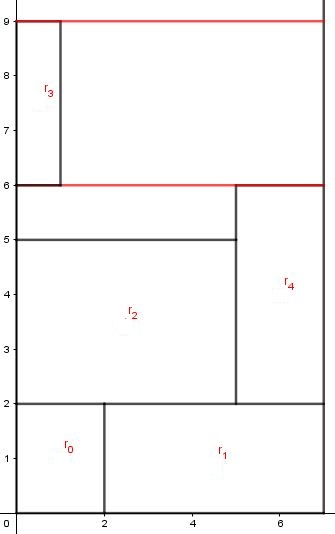
\includegraphics[width=0.7\linewidth]{grafica_ejemplo_solucion_GA.jpg}}
\caption{Representacion grafica de la solucion $I_0$}
\label{fig_1}
\end{figure}

Evaluaremos el desempeño de las soluciones en base a la menor altura de dicha solucion, por ejemplo, si tomamos la solucion $I_0$, su desempeño seria $f(I_0) = 9$ en cambio una solucion $I_1 = \{S_1,Mr_1\}$ con la forma $S_1 = (r_1,r_2,r_0,r_3,r_4), Mr_1 = (0,0,0,0,0)$, tendria un desempeño $f(I_1) = 11$, con dicho criterio de evaluacion podemos decir que $I_0$ es mejor solucion al problema que $I_1$ y por tanto es mas probable de ser seleccionada para reproducirse y volverse progenitora de individuos en siguientes generaciones.

\begin{figure}[H]
\centerline{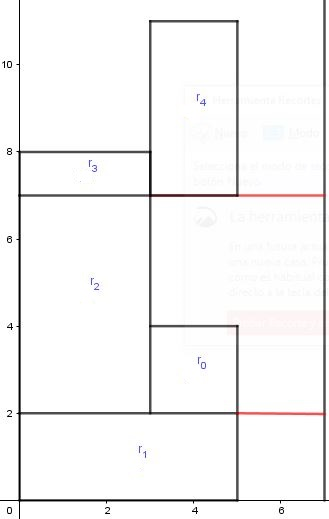
\includegraphics[width=0.7\linewidth]{grafica_ejemplo_solucion2_GA.jpg}}
\caption{Representacion grafica de la solucion $I_1$}
\label{fig_2}
\end{figure}

Supongamos ahora que vamos a reproducir ambas soluciones $I_0,I_1$. Recordemos que existia una probabilidad asociada a la mutacion como al evolucionar. Si dichas probabilidades no se cumplen (los hijos no evolucionan ni mutan) simplemente heredaran los genes de sus progenitores, el hijo $H_0 = I_0, H_1 = I_1$, los progenitores "pasarian" a la siguiente generacion sin cambios.

En caso de que se produzca un cruce (evolucion) el operador PMX trabajara con ambos progenitores de la siguiente forma: 
Se toma un intervalo aleatorio en el cromosoma de la solucion, por ejemplo $b = [1,3]$ en $I_0$ el rango abarcaria $S_0[1,2] = (r_0,r_1), Mr_0[1,2] = (0,0)$ y en $I_1$, $S_1[1,3] = (r_1,r_2), Mr_1[1,2] = (0,0)$.

Generamos dos hijos $H_0 = I_0, H_1 = I_1$, tomamos los genes del intervalo
$$H_0[1,2] = \{(r_0,r_1),(0,0)\}, H_1[1,2] = \{(r_1,r_2),(0,0)\}$$

Intercambiamos los genes con el progenitor opuesto:
$$H_0[1,2] = I_1[1,2] = \{(r_1,r_2),(0,0)\}, H_1[1,2] = I_0[1,2] = \{(r_0,r_1),(0,0)\}$$ 

Los hijos nos quedan de la forma: 
$$H_0=\{(r_1,r_2,r_2,r_4,r_3),(0,0,1,0,1)\}, H_1 = \{(r_0,r_1,r_0,r_3,r_4),(0,0,0,0,0)\}$$

Podemos ver que los rectangulos $r_2, r_0$ se encuentran repetidos en $H_0$ y $H_1$ respectivamente, para corregir esto tomamos aquellos genes repetidos que quedaron fuera del intervalo $b$ en este caso el tercer gen de cada cromosoma y lo reemplazamos por un rectangulo aleatorio faltante $r_0, r_2$ respectivamente, obteniendo como resultado:
$$H_0=\{(r_1,r_2,r_0,r_4,r_3),(0,0,0,0,1)\}, H_1 = \{(r_0,r_1,r_2,r_3,r_4),(0,0,0,0,0)\}$$

Ahora dado que al recuperar el rectangulo faltante en cada hijo, lo insertamos por defecto, es decir, sin rotar, tomaremos el tercer gen del cromosoma $Mr_i$ y lo reemplazaremos por un valor booleano aleatorio, nos quedaria de la siguiente forma:
$$H_0=\{(r_1,r_2,r_0,r_4,r_3),(0,0,0,0,1)\}, H_1 = \{(r_0,r_1,r_2,r_3,r_4),(0,0,1,0,0)\}$$

Suponiendo una mutacion en alguno de los hijos, $H_0$, simplemente permutamos dos genes y su valor booleano respectivo, por ejemplo intercambiamos $r_1,r_3$ y $m_0,m_4$ en $H_0$ obteniendo:
$$H_0=\{(r_3,r_2,r_0,r_4,r_1),(1,0,0,0,0)\}$$

Tambien mutaremos el cromosoma $M_0$ independiente de $S_0$, por ejemplo $m_0,m_1$:
$$H_0=\{(r_3,r_2,r_0,r_4,r_1),(0,1,0,0,0)\}$$

Con estas bases podemos encarar el problema de forma general, recordando: 
Un problema, $R = \{r_0,r_1,..,r_n\}$
Una poblacion inicial $P_0={i_0,i_1,...,i_k}$ donde cada individuo es de la forma:
$I_i = \{S_i,Mr_i\}$ donde $S_i = (r_0,r_1,..,r_n), Mr_i = (m_0, m_1,...,m_n)$, $|R| = |S_i| = |Mr_i|$

A cada inviduo $I_j \in P_i$ se lo evaluara en funcion a su altura total (se considerara o no el valor booleano respectivo a cada rectangulo, para evaluarlo rotado o no dependiendo si permitimos rotaciones en el algoritmo). Se los hara competir entre si de forma aleatoria, solo la mitad de la poblacion podra reproducirse, la nueva generacion obtenida $P_{i+1}$ tendra como individuos a los hijos de los progenitores que lograron reproducirse en la generacion anterior (algunos mutados o con cruzamiento). 

De esta manera la mayoria de individuos existentes son hijos de aquellos con mejor desempeño, aquellos con menor desempeño tendran menos probabilidades de reproducirse, pero nunca 0\% con esto evitamos la desaparicion de ciertas combinaciones interesantes logrando mas variedad en la poblacion que puede resultar en mejores soluciones inesperadas que no hubiesen ocurrido de haber descartado los individuos con menor desempeño.

El GA ira guardando la mejor solucion historica y los mejores puntajes de cada generacion, asi podemos ver como fue "evolucionando" la poblacion y cual fue la mejor solucion de todas. Una implementacion en Python de dicho algoritmo podemos encontrar en el apendice del informe, en esta implementacion podemos indicar si queremos o no habilitar la posibilidad de rotar los rectangulos.

\section{Resultados y estadisticas} % o Experimentos realizados o Estudio realizado
 
Probamos el algoritmo en seis instancias diferente del problema, cada instancia fue ejecutada $20$ veces con diferentes semillas $i=0,1...,19$. A continuacion presentamos las estadisticas de las mejores soluciones sin rotacion y con rotacion:



%\subsection*{spp9a.txt}
%\noindent \textbf{Problema}: W = 15 [(4, 15), (15, 3), (6, 6), (3, 12), (4, 6), (2, 8), (8, 2), (3, 5), (10, 3)]\newline
%\newline
%\textbf{AG sin rotacion}\newline
%Media: 27.6\newline
%Mediana: 27.0\newline
%Desviacion: 0.9165151389911679\newline
%\newline
%\textbf{AG con rotacion}\newline
%Media con rotacion : 23.25\newline
%Mediana con rotacion : 23.0\newline
%Desviacion con rotacion : 0.9420721840708386
\label{sec:Estadisticas}%
En esta seccion mostraremos algunos resultados obtenidos de las multiples ejecuciones de diferentes instancias del problema.%
También, posteriormente un analisis, comparación y evaluación de estos resultados%
\subsection{Resultados instancia: spp9a.txt}%
\label{subsec:Resultadosinstanciaspp9a.txt}%
Problema : W=15{[}(4, 15), (15, 3), (6, 6), (3, 12), (4, 6), (2, 8), (8, 2), (3, 5), (10, 3){]} \newline%
%
 Algoritmo sin Rotación : %
\begin{itemize}%
\item%
Promedio : 27.6%
\item%
Mediana : 27.0%
\item%
Desviación estandar : 0.9165151389911679%
\end{itemize}

%Grafico
\begin{figure}[H]
\centerline{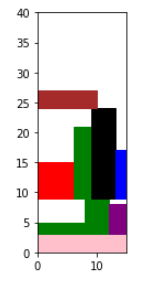
\includegraphics[width=0.5\linewidth]{1_sin_rotar.jpg}}
\caption{Grafico de Instancia SPPA9a }
\label{fig_1}
\end{figure}

Algoritmo con Rotación : %
\begin{itemize}%
\item%
Promedio : 23.25%
\item%
Mediana : 23.0%
\item%
Desviación estandar : 0.9420721840708386%
\end{itemize}%

%Grafico
\begin{figure}[H]
\centerline{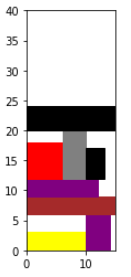
\includegraphics[width=0.5\linewidth]{1_con_rotar.jpg}}
\caption{Grafico de Instancia SPPA9a con rotacion }
\label{fig_2}
\end{figure}
%Rotacion

\subsection{Resultados instancia: spp9b.txt}%
\label{subsec:Resultadosinstanciaspp9b.txt}%
Problema : W=15{[}(4, 15), (15, 3), (6, 6), (3, 12), (3, 8), (2, 8), (8, 2), (3, 5), (10, 3){]} \newline%
%
 Algoritmo sin Rotación : %
\begin{itemize}%
\item%
Promedio : 27.3%
\item%
Mediana : 27.0%
\item%
Desviación estandar : 0.714142842854285%
\end{itemize}

%Grafico
\begin{figure}[H]
\centerline{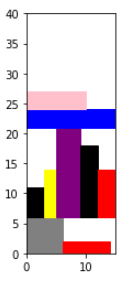
\includegraphics[width=0.5\linewidth]{2_sin_rotar.jpg}}
\caption{Grafico de Instancia SPPA9b }
\label{fig_3}
\end{figure} 

%
Algoritmo con Rotación : %
\begin{itemize}%
\item%
Promedio : 23.25%
\item%
Mediana : 23.0%
\item%
Desviación estandar : 0.8874119674649424%
\end{itemize}%

%Grafico
\begin{figure}[H]
\centerline{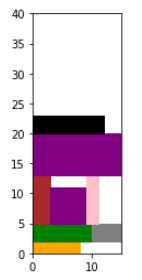
\includegraphics[width=0.5\linewidth]{2_con_rotar.jpg}}
\caption{Grafico de Instancia SPPA9b con rotacion}
\label{fig_4}
\end{figure} 


\subsection{Resultados instancia: spp10.txt}%
\label{subsec:Resultadosinstanciaspp10.txt}%
Problema : W=20{[}(5, 11), (9, 8), (2, 8), (3, 6), (4, 9), (6, 8), (4, 7), (9, 8), (3, 11), (2, 11){]} \newline%
%
 Algoritmo sin Rotación : %
\begin{itemize}%
\item%
Promedio : 26.8%
\item%
Mediana : 27.0%
\item%
Desviación estandar : 0.39999999999999997%
\end{itemize}

%Grafico
\begin{figure}[H]
\centerline{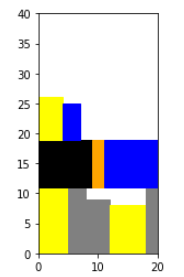
\includegraphics[width=0.5\linewidth]{3_sin_rotar.jpg}}
\caption{Grafico de Instancia SPPA10 }
\label{fig_5}
\end{figure} 


%
Algoritmo con Rotación : %
\begin{itemize}%
\item%
Promedio : 24.9%
\item%
Mediana : 25.0%
\item%
Desviación estandar : 0.9433981132056604%
\end{itemize}%

%Grafico
\begin{figure}[H]
\centerline{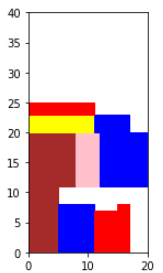
\includegraphics[width=0.5\linewidth]{3_con_rotar.jpg}}
\caption{Grafico de Instancia SPPA10 con rotacion}
\label{fig_6}
\end{figure} 


\subsection{Resultados instancia: spp11.txt}%
\label{subsec:Resultadosinstanciaspp11.txt}%
Problema : W=20{[}(4, 13), (7, 8), (10, 5), (2, 8), (6, 7), (3, 8), (1, 12), (4, 7), (4, 4), (6, 12), (4, 8){]} \newline%
%
 Algoritmo sin Rotación : %
\begin{itemize}%
\item%
Promedio : 26.7%
\item%
Mediana : 26.0%
\item%
Desviación estandar : 0.9539392014169457%
\end{itemize}


%Grafico
\begin{figure}[H]
\centerline{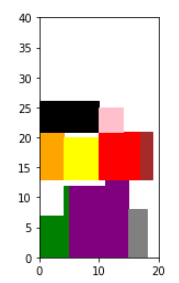
\includegraphics[width=0.5\linewidth]{4_sin_rotar.jpg}}
\caption{Grafico de Instancia SPPA11}
\label{fig_7}
\end{figure} 


%
Algoritmo con Rotación : %
\begin{itemize}%
\item%
Promedio : 25.4%
\item%
Mediana : 25.5%
\item%
Desviación estandar : 1.2409673645990857%
\end{itemize}%

%Grafico
\begin{figure}[H]
\centerline{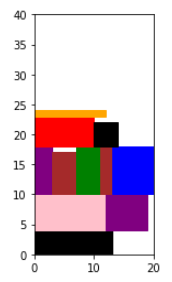
\includegraphics[width=0.5\linewidth]{4_con_rotar.jpg}}
\caption{Grafico de Instancia SPPA11 con rotacion}
\label{fig_8}
\end{figure} 



\subsection{Resultados instancia: spp12.txt}%
\label{subsec:Resultadosinstanciaspp12.txt}%
Problema : W=20{[}(3, 6), (5, 8), (4, 5), (10, 8), (7, 4), (6, 3), (8, 8), (4, 6), (18, 3), (2, 3), (3, 10), (9, 2){]} \newline%
%
 Algoritmo sin Rotación : %
\begin{itemize}%
\item%
Promedio : 26.9%
\item%
Mediana : 27.0%
\item%
Desviación estandar : 0.8306623862918073%
\end{itemize}

%Grafico
\begin{figure}[H]
\centerline{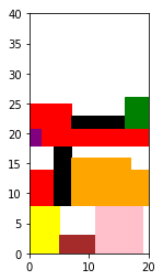
\includegraphics[width=0.5\linewidth]{5_sin_rotar.jpg}}
\caption{Grafico de Instancia SPPA12 }
\label{fig_9}
\end{figure} 


%
Algoritmo con Rotación : %
\begin{itemize}%
\item%
Promedio : 25.1%
\item%
Mediana : 25.0%
\item%
Desviación estandar : 0.8306623862918073%
\end{itemize}%

%Grafico
\begin{figure}[H]
\centerline{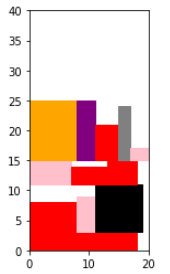
\includegraphics[width=0.5\linewidth]{5_con_rotar.jpg}}
\caption{Grafico de Instancia SPPA12  con rotacion}
\label{fig_10}
\end{figure} 


\subsection{Resultados instancia: spp13.txt}%
\label{subsec:Resultadosinstanciaspp13.txt}%
Problema : W=20{[}(7, 5), (1, 8), (5, 9), (9, 3), (2, 16), (9, 7), (5, 9), (5, 3), (4, 9), (3, 7), (2, 7), (9, 3), (2, 16){]} \newline%
%
 Algoritmo sin Rotación : %
\begin{itemize}%
\item%
Promedio : 32.1%
\item%
Mediana : 32.0%
\item%
Desviación estandar : 1.1789826122551597%
\end{itemize}

%Grafico
\begin{figure}[H]
\centerline{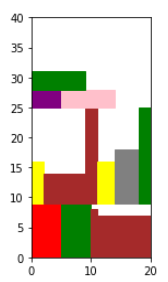
\includegraphics[width=0.5\linewidth]{6_sin_rotar.jpg}}
\caption{Grafico de Instancia SPPA13 }
\label{fig_11}
\end{figure} 

%
Algoritmo con Rotación : %
\begin{itemize}%
\item%
Promedio : 26.45%
\item%
Mediana : 26.5%
\item%
Desviación estandar : 1.532155344604456%
\end{itemize}

%Grafico
\begin{figure}[H]
\centerline{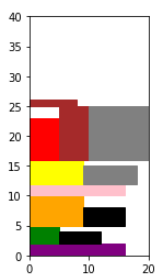
\includegraphics[width=0.5\linewidth]{6_con_rotar.jpg}}
\caption{Grafico de Instancia SPPA13 con rotacion }
\label{fig_12}
\end{figure} 

Podemos observar como el permitir rotaciones de rectangulos se aprovecha mejor es espacio de la tira para todas las instancias, reduciendo asi la cantidad de desperdicio de forma sustancial. Para este tipo de problemas de alta complejidad vemos que los algoritmos geneticos tienen un desempeño mas que aceptable, siendo una excelente forma de encarar este tipo de problemas.


\section{Conclusiones}
Dada la simplesa de los algoritmos y su desempeño a la hora de encontrar una solucion eficiente, las metaheuristicos poblacionales, en este caso Algoritmos Geneticos, son una excelente forma de atacar problemas de complejidad NP hard cuya funcion de evaluacion sea simple (minimo valor posible) como es el caso de SPP, problema que surje en distintas areas ademas de las obvias como pueden ser aprovechamiento de material (madera, vidrio, metal,etc) como en la computacion donde se modelan jobs que requieren una parte contigua de la memoria durante un período de tiempo determinado entre otros.

En conclusion, los GA, son una prometedora herramienta para la industria.

%------------------------------------------------ 
\section*{Agradecimientos}
Prof. Guillermo Leguizamon

%----------------------------------------------------------------------------------------
%	Listado de bibliografía consultada / Puede incluír sitios web
%----------------------------------------------------------------------------------------

\begin{thebibliography}{99} % Bibliography - this is intentionally simple in this template
\bibitem0.\t[Clinton Sheppard, 2018]{}Genetic Algorithms with Python
\bibitem1.\t[Wikipedia]{} \url{https://en.wikipedia.org/wiki/Strip_packing_problem}
\bibitem2.\t[Wikipedia]{}\url{https://en.wikipedia.org/wiki/Genetic_algorithm}
\bibitem2.\t[Wikipedia]{}\url{https://en.wikipedia.org/wiki/Crossover_(genetic_algorithm)}
\bibitem3.\t[Universidad de Liverpool]{} Efficient Algorithms for 2-D Rectangle packing \url{https://cgi.csc.liv.ac.uk/~epa/surveyhtml.html}

\end{thebibliography} 
 
\section{Código del Algoritmo}
\begin{lstlisting}[language=Python]
def init_population(pop_size,individuals,rotacion):
    list=np.arange(individuals)
    if(rotacion):
      #inicializacion con la mascara de booleanos aleatoria
      pop=np.array([(np.random.permutation(list).tolist(),                      
                   [random.choice([True, False]) for j in range(individuals)]) 
                   for i in range(pop_size)])                                 
    else:
      pop=np.array([(np.random.permutation(list).tolist(),
      			   [False for j in range(individuals)]) 
      			   for i in range(pop_size)])
    return pop

def calculate_fitness(population,rectangles):
    #Ancho maximo de la tira
    global W
    shape=np.shape(population)
    pop_size=shape[0]
    ind=shape[2]
    scores=[]#fitness de la poblacion
    #Recorre todas las soluciones de la poblacion
    for i in range(pop_size):
        ancho_nivel=0
        alto_max=0
        niveles=[]#cantidad de niveles, guardo altura de cada nivel
        #Recorre el orden de los rectangulos de las soluciones
        for j in range(ind):
            #Obtiene ancho y largo del rectangulo
            indx=population[i,0][j]
            #si el booleano correspondiente es verdadero lo roto
            if population[i,1][j]: 
              r_i=obtener_rotado(rectangles[indx])
            else:
              r_i=rectangles[indx]
            ancho_r=r_i.width
            alto_r=r_i.height
            w=ancho_r+ancho_nivel
            #Si al agregar el rectangulo no nos pasamos del ancho
            #Se agrega el rectangulo al nivel actual de la sol.
            #Se actualiza el alto de ser necesario
            if w<=W:
                ancho_nivel=w
                if alto_r>alto_max:
                    alto_max=alto_r
            else:
                niveles.append(alto_max)
                ancho_nivel=ancho_r
                alto_max=alto_r
        niveles.append(alto_max)
        #Puntaje es la suma del largo de niveles, menor mejor
        scores.append(np.sum(niveles))
    return scores

def ejecucion_ga(args):
  #with_rotation es un booleano

  best_score_global = float('inf')
  best_solution = []
  for generation in range(MAXG):
        new_population=[]
        if best_score < best_score_global: #Mejor individuo historico
          best_score_global = best_score
          best_solution = pop[np.argmin(scores)][:]
        for i in range(int(PSIZE/2)):
            parent_1 = select_individual_by_tournament(pop, scores)
            parent_2 = select_individual_by_tournament(pop, scores)
            #Evolucion
            if np.random.random()<PC:
                child_1, child_2 = PMX(parent_1, parent_2,rotacion)
            else:
                child_1=parent_1
                child_2=parent_2
            #Mutacion
            if np.random.random()<PM:
                swap_mutation(child_1,child_2,rotacion)
            new_population.append(child_1)
            new_population.append(child_2)
        pop=np.array(new_population)
        scores=calculate_fitness(pop,rectangles)
        best_score=np.min(scores)
        best_scores_progress.append(best_score)
  return best_score_global, best_solution

def select_individual_by_tournament(population, scores):
    # Get population size
    population_size = len(scores)
    # Pick individuals for tournament
    fighter_1 = random.randint(0, population_size-1)
    fighter_2 = random.randint(0, population_size-1)
    while(fighter_1==fighter_2):
        fighter_2=random.randint(0,population_size-1)
    # Get fitness score for each
    fighter_1_fitness = scores[fighter_1]
    fighter_2_fitness = scores[fighter_2]
    # Identify undividual with highest fitness
    # Fighter 1 will win if score are equal
    if fighter_1_fitness <= fighter_2_fitness:
        winner = fighter_1
    else:
        winner = fighter_2
    # Return the chromsome of the winner
    return population[winner, :]

def PMX(parent_1, parent_2,rotacion):
    # Get length of chromosome
    chromosome_length = len(parent_1[0])
    p_1=np.asarray(parent_1)
    p_2=np.asarray(parent_2)

    # Pick points, avoding ends of chromsome 
    point_1 = random.randint(1,chromosome_length-2)
    #-2 para que no haya problemas con el max
    point_2 = random.randint(point_1+1,chromosome_length-1)#Al menos 2
    b=np.arange(point_1,point_2+1) #Intervalo b para intercambio de genes

    child_1=np.array(parent_1)
    child_1[0][b]=p_2[0][b]
    child_1[1][b]=p_2[1][b]
    child_2=np.array(parent_2)
    child_2[0][b]=p_1[0][b]
    child_2[1][b]=p_1[1][b]
    
    corregir_faltantes(child_1,p_2,p_1,b,rotacion)
    corregir_faltantes(child_2,p_1,p_2,b,rotacion)
    return child_1, child_2

def corregir_faltantes(child,p_1,p_2,b,rotacion):
  chromosome_length = len(p_1[0])
  faltantes=[i for i in range(chromosome_length) 
  			if i not in child[0]]
  if faltantes:
    indices=[i for i in range(chromosome_length) 
    		if p_2[0][i] in p_1[0][b] and i not in b]
    child[0][indices]=np.random.choice(faltantes,len(indices),replace=False)
    child[1][indices] = False
    if rotacion:
      #El rectangulo faltante puede venir o no rotado 
      child[1][indices]=random.choice([True, False]) 
  
def swap_mutation(ind_1,ind_2,rotacion):
    global PM
    chr_len=len(ind_1[0])

    i_1=random.randint(0,chr_len-1)
    i_2=random.randint(0,chr_len-1)
    while(i_2==i_1):
        i_2=random.randint(0,chr_len-1)

    swap(ind_1[0][i_1],ind_1[0][i_2])
    swap(ind_2[0][i_1],ind_2[0][i_2])
    #Si rotacion falso entonces la mascara de booleanos es (0,0,..0)
    #No tiene sentido intercambiarla  
    if rotacion:
      #Al mover el rectangulo no se lo rota
      #Los booleanos deben intercambiarse
      swap(ind_1[1][i_1],ind_1[1][i_2])
      swap(ind_2[1][i_1],ind_2[1][i_2])
      #Intercambio de dos booleanos aleatorios
      i_1=random.randint(0,chr_len-1)
      i_2=random.randint(0,chr_len-1)
      while(i_2==i_1):
          i_2=random.randint(0,chr_len-1)
      
      swap(ind_1[1][i_1],ind_1[1][i_2])
      swap(ind_2[1][i_1],ind_2[1][i_2])
    return ind_1,ind_2

\end{lstlisting}
\newpage
\tableofcontents
\end{document}